% *********************************************************************
% © 2010–2022 Jeremy Sylvestre
%
% Permission is granted to copy, distribute and/or modify this document
% under the terms of the GNU Free Documentation License, Version 1.3 or
% any later version published by the Free Software Foundation; with no
% Invariant Sections, no Front-Cover Texts, and no Back-Cover Texts. A
% copy of the license is included in the appendix entitled “GNU Free
% Documentation License” that appears in the output document of this
% PreTeXt source code. All trademarks™ are the registered® marks of
% their respective owners.
%
% *********************************************************************

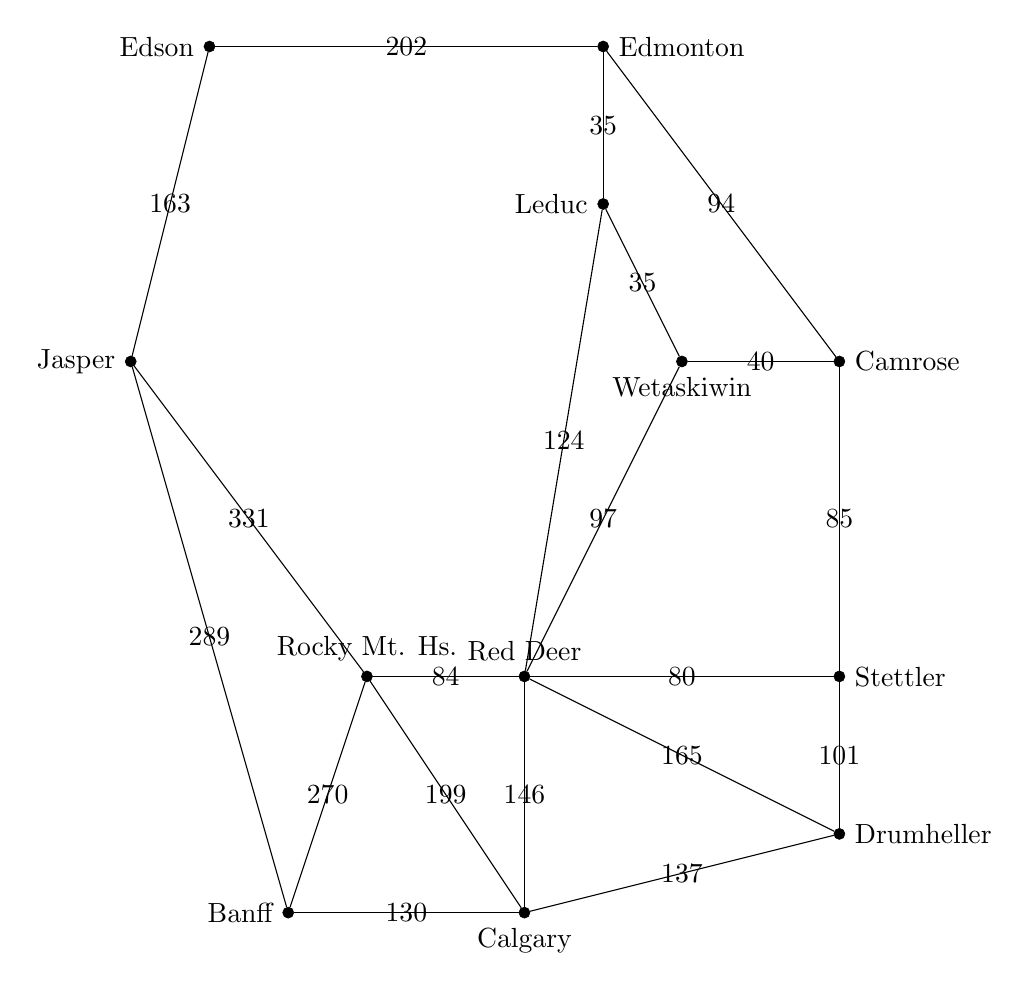
\begin{tikzpicture}[
	vertex/.style={ circle, draw, very thin, fill, inner sep=0pt, minimum size=4pt },
	vertexg/.style={ black!40!white, circle, draw, very thin, fill, inner sep=0pt, minimum size=4pt },
	vertexo/.style={ circle, draw, very thin, inner sep=0pt, minimum size=4pt }
]

\node at (-3,4) (e) [vertex,label=right:Edmonton] {};
\node at (0,0) (c) [vertex,label=right:Camrose] {};
\draw (c) to node {94} (e);
\node at (-2,0) (w) [vertex,label=below:Wetaskiwin] {};
\draw (c) to node {40} (w);
\node at (-3,2) (l) [vertex,label=left:Leduc] {};
\draw (w) to node {35} (l);
\node at (-4,-4) (rd) [vertex,label=above:Red Deer] {};
\draw (l) to node {124} (rd);
\node at (0,-4) (st) [vertex,label=right:Stettler] {};
\draw (st) to node {85} (c);
\node at (0,-6) (dr) [vertex,label=right:Drumheller] {};
\draw (dr) to node {101} (st);
\node at (-4,-7) (cg) [vertex,label=below:Calgary] {};
\draw (cg) to node {146} (rd);
\node at (-7,-7) (bf) [vertex,label=left:Banff] {};
\draw (bf) to node {130} (cg);
\node at (-9,0) (js) [vertex,label=left:Jasper] {};
\draw (js) to node {289} (bf);
\node at (-8,4) (eds) [vertex,label=left:Edson] {};
\draw (eds) to node {163} (js);
\node at (-6,-4) (rmh) [vertex,label=above:Rocky Mt. Hs.] {};
\draw (rmh) to node {84} (rd);
\draw (l) to node {35} (e);
\draw (w) to node {97} (rd);
\draw (rd) to node {80} (st);
\draw (rd) to node {165} (dr);
\draw (dr) to node {137} (cg);
\draw (e) to node {202} (eds);
\draw (js) to node {331} (rmh);
\draw (rmh) to node {270} (bf);
\draw (rmh) to node {199} (cg);

\end{tikzpicture}
